\documentclass[11pt,letterpaper]{article}
\usepackage[T1]{fontenc}
\usepackage[scaled]{helvet}
\renewcommand{\familydefault}{\sfdefault}
\usepackage{amsmath,amssymb}
\usepackage[margin=0.8in,bottom=0.9in]{geometry}
\usepackage[most]{tcolorbox}
\usepackage{tikz}
\usetikzlibrary{calc}
\usepackage{enumitem}
\usepackage{array}
\usepackage{needspace}
\usepackage{fancyhdr}
\usepackage{pifont}

% ---- Palette "F. Bright & Playful" ----
\definecolor{fmtitle}{HTML}{3D2C8D}
\definecolor{fmkey}{HTML}{0096C7}
\definecolor{fmwatch}{HTML}{2BB673}
\definecolor{fmturn}{HTML}{F4A100}
\definecolor{fmmistake}{HTML}{EF476F}
\definecolor{fmnotice}{HTML}{9B5DE5}
\definecolor{fmgray}{HTML}{6B6B6B}

\pagestyle{fancy}
\fancyhf{}
\renewcommand{\headrulewidth}{0pt}
\fancyfoot[C]{\footnotesize\color{fmgray}\textcopyright\ 2026 FangMath. All rights reserved.}
\fancyfoot[R]{\footnotesize\color{fmgray}\thepage}
\setlength{\parindent}{0pt}
\setlength{\parskip}{3pt}

\newcommand{\badge}[1]{\colorbox{fmtitle}{\color{white}\bfseries\small\ #1\ }}
\newcommand{\leveltag}[2]{\colorbox{#1}{\color{white}\bfseries\scriptsize\ #2\ }}
\newcommand{\LE}{\leveltag{fmwatch}{EASY}}
\newcommand{\LM}{\leveltag{fmturn}{MEDIUM}}
\newcommand{\LH}{\leveltag{fmmistake}{HARD}}

\newcommand{\sectionbar}[2]{\needspace{6cm}\par\vspace{4mm}
  \begin{tcolorbox}[enhanced,colback=fmtitle,colframe=fmtitle,arc=2mm,
    left=4mm,top=1.5mm,bottom=1.5mm]
  \color{white}\bfseries\large #1\hfill{\normalsize\mdseries #2}
  \end{tcolorbox}}

\newtcolorbox{keyidea}{enhanced,breakable,colback=white,colframe=fmkey,boxrule=1pt,arc=2mm,
  title={Key Idea},coltitle=fmkey,fonttitle=\bfseries,
  attach boxed title to top left={xshift=4mm,yshift=-2mm},
  boxed title style={colback=white,colframe=fmkey,boxrule=0.9pt}}
\newtcolorbox{watchme}{enhanced,colback=white,colframe=fmwatch,boxrule=1pt,arc=2mm,
  title={Watch Me --- Worked Example},coltitle=fmwatch,fonttitle=\bfseries,
  attach boxed title to top left={xshift=4mm,yshift=-2mm},
  boxed title style={colback=white,colframe=fmwatch,boxrule=0.9pt}}
\newtcolorbox{mistakebox}{enhanced,breakable,colback=white,colframe=fmmistake,boxrule=1pt,arc=2mm,
  title={Common Mistake},coltitle=fmmistake,fonttitle=\bfseries,
  attach boxed title to top left={xshift=4mm,yshift=-2mm},
  boxed title style={colback=white,colframe=fmmistake,boxrule=0.9pt}}
\newtcolorbox{yourturn}{enhanced,breakable,colback=white,colframe=fmturn,boxrule=1pt,arc=2mm,
  title={Your Turn},coltitle=fmturn,fonttitle=\bfseries,
  attach boxed title to top left={xshift=4mm,yshift=-2mm},
  boxed title style={colback=white,colframe=fmturn,boxrule=0.9pt}}
\newtcolorbox{answerbox}[1]{enhanced,breakable,colback=white,colframe=fmwatch,boxrule=1pt,arc=2mm,
  title={#1},coltitle=fmwatch,fonttitle=\bfseries,
  attach boxed title to top left={xshift=4mm,yshift=-2mm},
  boxed title style={colback=white,colframe=fmwatch,boxrule=0.9pt}}

\newcommand{\work}[1]{\par\vspace{#1}}
\setlist[enumerate]{itemsep=2pt,topsep=3pt}

% ---------------- extra boxes ----------------
\newtcolorbox{notebox}{enhanced,breakable,colback=white,colframe=fmnotice,boxrule=1pt,arc=2mm,
  title={Notice},coltitle=fmnotice,fonttitle=\bfseries,
  attach boxed title to top left={xshift=4mm,yshift=-2mm},
  boxed title style={colback=white,colframe=fmnotice,boxrule=0.9pt}}
\newtcolorbox{exbox}{enhanced,colback=white,colframe=fmwatch,boxrule=0.8pt,arc=2mm,
  title={Example},coltitle=fmwatch,fonttitle=\bfseries\small,
  attach boxed title to top left={xshift=4mm,yshift=-2mm},
  boxed title style={colback=white,colframe=fmwatch,boxrule=0.8pt},fontupper=\small}
\newcommand{\topicbar}[1]{\needspace{4.5cm}\par\vspace{5mm}
  \begin{tcolorbox}[enhanced,colback=fmtitle,colframe=fmtitle,arc=2mm,left=4mm,top=1.5mm,bottom=1.5mm]
  \color{white}\bfseries\large #1
  \end{tcolorbox}}
\usepackage{multicol}

% ---------------- practice layout ----------------
\newcommand{\workline}{\par\vspace{7mm}{\color{gray!55}\rule{\linewidth}{0.4pt}}}
\newcommand{\worklines}[1]{\foreach \i in {1,...,#1}{\workline}}
\newcommand{\prob}[3]{\needspace{#3}\par\vspace{3mm}{\color{fmturn}\bfseries #1.}\ #2\par}
\newcommand{\ansline}{\par\vspace{4mm}\hfill\textbf{Answer:}\ \rule{5cm}{0.4pt}\par}
\newcommand{\keyitem}[3]{\needspace{3.2cm}\par\vspace{2mm}
  \begin{tcolorbox}[enhanced,colback=white,colframe=fmwatch!60,boxrule=0.6pt,arc=1.5mm,left=3mm,top=1.5mm,bottom=1.5mm]
  {\color{fmwatch}\bfseries #1.}\quad\small #2\par\vspace{1mm}
  \normalsize\textbf{Answer: #3}
  \end{tcolorbox}}


\usetikzlibrary{arrows.meta}
\providecommand{\iskey}{0}
% fill-in blank: line for students, pink answer in the key
\newcommand{\fb}[2][2.6cm]{\ifnum\iskey=1 \underline{\makebox[#1][c]{\color{fmmistake}\bfseries #2}}\else\underline{\makebox[#1]{}}\fi}
% answer line for practice problems
\newcommand{\pans}[2][3.2cm]{\ifnum\iskey=1 \underline{\makebox[#1][c]{\color{fmmistake}\bfseries #2}}\else\rule{#1}{0.4pt}\fi}
\newcommand{\vid}[1]{{\color{fmgray}\small\textit{\ding{43} Video: #1}}}
\newcommand{\pt}[2]{\fill (#1) circle (2.2pt) node[above=1pt,font=\small]{$#2$};}

\usetikzlibrary{decorations.pathreplacing}
% three points on a segment with lengths written above the pieces: #1,#2,#3 letters; #4,#5 piece labels; #6 whole label (below)
\newcommand{\threept}[6]{\begin{tikzpicture}[x=1cm]\draw[thick] (0,0)--(3.6,0);
\fill (0,0) circle(2.2pt) node[below=2pt,font=\small]{$#1$} (1.4,0) circle(2.2pt) node[below=2pt,font=\small]{$#2$} (3.6,0) circle(2.2pt) node[below=2pt,font=\small]{$#3$};
\node[above,font=\small] at (0.7,0.02){#4};\node[above,font=\small] at (2.5,0.02){#5};
\if\relax\detokenize{#6}\relax\else\draw[gray,decorate,decoration={brace,amplitude=4pt,mirror}] (0,-0.45)--(3.6,-0.45) node[midway,below=4pt,font=\small]{#6};\fi
\end{tikzpicture}}
\newcommand{\sdp}[3]{\begin{minipage}[t][2.4cm]{0.48\linewidth}{\color{fmturn}\bfseries #1.}\ #2\par\vfill\hfill \pans[3.6cm]{#3}\end{minipage}}
\newcommand{\figp}[4]{\begin{minipage}[t]{0.48\linewidth}{\color{fmturn}\bfseries #1.}\ #2\par\vspace{1mm}\centering #3\par\vspace{2mm}\raggedleft \pans[2.6cm]{#4}\end{minipage}}
\newcommand{\algp}[3]{\begin{minipage}[t][4.6cm]{0.48\linewidth}{\color{fmturn}\bfseries #1.}\ #2\par\vfill\hfill \pans[4.2cm]{#3}\end{minipage}}


% ch2: long key answers wrap inside their column instead of running into the next one
\newlength{\pw}
\renewcommand{\pans}[2][3.2cm]{\ifnum\iskey=1 \settowidth{\pw}{\bfseries #2}\ifdim\pw>#1 \parbox[b]{#1}{\raggedleft\color{fmmistake}\bfseries\small #2}\else\underline{\makebox[#1][c]{\color{fmmistake}\bfseries #2}}\fi\else\rule{#1}{0.4pt}\fi}
\begin{document}
\ifnum\iskey=1 \colorbox{fmwatch}{\color{white}\bfseries\small\ ANSWER KEY\ }\else\badge{PRACTICE}\fi\hfill{\small\color{fmgray}Geometry \textperiodcentered\ Lesson 2.5}\par\vspace{4mm}
{\color{fmtitle}\LARGE\bfseries Two-Column Proofs --- Practice\ifnum\iskey=1 \ --- Answer Key\fi}\par\vspace{1mm}
{\color{fmgray}A worked example comes before each type. Fill in every missing statement and reason.}\par\vspace{3mm}
Name: \rule{6cm}{0.4pt}\hspace{1cm}Date: \rule{3.5cm}{0.4pt}\par\vspace{2mm}
\newcommand{\rsn}[1]{\pans[6.2cm]{#1}}
\newcommand{\stm}[1]{\pans[3.6cm]{#1}}
\newenvironment{pf}{\par\vspace{1mm}\renewcommand{\arraystretch}{1.9}\begin{tabular}{@{}p{6.2cm}|l@{}}\textbf{Statements} & \textbf{Reasons}\\ \hline}{\end{tabular}\par\vspace{2mm}}

\needspace{6cm}\topicbar{Type 1 \quad Algebra Proofs}
\begin{watchme}Given: $\tfrac{x}{2} + 3 = 7$ \quad Prove: $x = 8$\par
1.\ $\tfrac{x}{2} + 3 = 7$ \ (Given) \quad 2.\ $\tfrac{x}{2} = 4$ \ (Subtraction Property of Equality) \quad 3.\ $x = 8$ \ (Multiplication Property of Equality)\end{watchme}
\needspace{5cm}{\color{fmturn}\bfseries 1.}\ Given: $4x + 9 = 25$ \quad Prove: $x = 4$
\begin{pf}
1.\ $4x + 9 = 25$ & Given\\
2.\ \stm{$4x = 16$} & \rsn{Subtraction Property of Equality}\\
3.\ $x = 4$ & \rsn{Division Property of Equality}\\
\end{pf}
\needspace{6cm}{\color{fmturn}\bfseries 2.}\ Given: $3(x - 1) = 2x + 5$ \quad Prove: $x = 8$
\begin{pf}
1.\ $3(x - 1) = 2x + 5$ & Given\\
2.\ $3x - 3 = 2x + 5$ & \rsn{Distributive Property}\\
3.\ \stm{$x - 3 = 5$} & \rsn{Subtraction Property of Equality}\\
4.\ $x = 8$ & \rsn{Addition Property of Equality}\\
\end{pf}

\needspace{7cm}\topicbar{Type 2 \quad Segment Proofs}
\begin{watchme}\begin{minipage}[c]{0.3\linewidth}\centering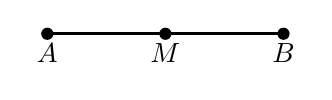
\begin{tikzpicture}\draw[very thick] (0,0)--(3,0); \foreach \x/\l in {0/A,1.5/M,3/B} \fill (\x,0) circle(2.2pt) node[below]{$\l$};\end{tikzpicture}\end{minipage}\hfill
\begin{minipage}[c]{0.66\linewidth}Given: $M$ is the midpoint of $\overline{AB}$. \ Prove: $AM = \tfrac12 AB$.\par
1.\ $M$ is the midpoint (Given) \ 2.\ $AM = MB$ (Def.\ of midpoint) \ 3.\ $AM + MB = AB$ (Segment Addition) \ 4.\ $AM + AM = AB$ (Substitution) \ 5.\ $2AM = AB$ (Simplify) \ 6.\ $AM = \tfrac12 AB$ (Division Prop.)\end{minipage}\end{watchme}
\needspace{7cm}{\color{fmturn}\bfseries 3.}\ \begin{minipage}[t]{0.55\linewidth}Given: $PQ = RS$ \quad Prove: $PR = QS$\end{minipage}\hfill\begin{minipage}[t]{0.38\linewidth}\centering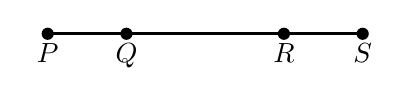
\begin{tikzpicture}\draw[very thick] (0,0)--(4,0); \foreach \x/\l in {0/P,1/Q,3/R,4/S} \fill (\x,0) circle(2.2pt) node[below]{$\l$};\end{tikzpicture}\end{minipage}
\begin{pf}
1.\ $PQ = RS$ & Given\\
2.\ $QR = QR$ & \rsn{Reflexive Property}\\
3.\ \stm{$PQ + QR = QR + RS$} & \rsn{Addition Property of Equality}\\
4.\ $PQ + QR = PR$, \ $QR + RS = QS$ & \rsn{Segment Addition Postulate}\\
5.\ $PR = QS$ & \rsn{Substitution Property}\\
\end{pf}

\needspace{7cm}\topicbar{Type 3 \quad Angle Proofs}
\begin{watchme}Given: $\overrightarrow{BD}$ bisects $\angle ABC$. \ So $m\angle ABD = m\angle DBC$ --- reason: \textbf{Definition of angle bisector}.\par
Then $m\angle ABD + m\angle DBC = m\angle ABC$ --- reason: \textbf{Angle Addition Postulate}.\end{watchme}
\needspace{6.5cm}{\color{fmturn}\bfseries 4.}\ Given: $m\angle 1 = m\angle 3$ \quad Prove: $m\angle ABD = m\angle CBE$ \quad {\small($\angle ABD$ is made of $\angle 1$ and $\angle 2$; $\angle CBE$ is made of $\angle 2$ and $\angle 3$.)}
\begin{pf}
1.\ $m\angle 1 = m\angle 3$ & Given\\
2.\ $m\angle 2 = m\angle 2$ & \rsn{Reflexive Property}\\
3.\ $m\angle 1 + m\angle 2 = m\angle 2 + m\angle 3$ & \rsn{Addition Property of Equality}\\
4.\ $m\angle 1 + m\angle 2 = m\angle ABD$ & \rsn{Angle Addition Postulate}\\
5.\ $m\angle 2 + m\angle 3 = m\angle CBE$ & \rsn{Angle Addition Postulate}\\
6.\ \stm{$m\angle ABD = m\angle CBE$} & \rsn{Substitution Property}\\
\end{pf}

\needspace{5cm}\topicbar{Type 4 \quad Find the Mistake}
\begin{watchme}A student wrote ``$\angle 1 \cong \angle 2$ \ --- \ Reason: they look the same.'' \quad That is not a reason. Use a given, definition, property, postulate or theorem.\end{watchme}
\needspace{3.4cm}\noindent\sdp{5}{Step: ``$2x = 10 \Rightarrow x = 5$. \ Reason: Subtraction Property.'' Fix the reason.}{Division Property of Equality}\hfill\sdp{6}{\LH\ Step: ``$AB = AB$. \ Reason: Symmetric Property.'' Fix the reason.}{Reflexive Property}\par
\end{document}
